\label{comparison:implementations}
\section{Aktuelle Implementierungen}
Für den Vergleich wurden Kafka und RabbitMQ gewählt, da sie in den letzten
Jahren am meisten Aufmerksamkeit erhalten haben. Dies ist zu sehen in
Darstellung \ref{searchinterest}, die das Volumen der jeweiligen
Suchanfragen für Implementierungen auf der Google Websuche zeigt.

In den letzten Jahren gab es auf dem Gebiet viele Neuentwicklungen, wie
beispielsweise NSQ. Dieses funktioniert komplett ohne zentrale Instanz als
Peer-to-Peer Ansatz. NSQ wird mit den restlichen Implementierungen verglichen,
um die ansatzbedingten Unterschiede aufzuzeigen und die Allgemeingültigkeit des
Katalogs zu demonstrieren. Es wird statt ZeroMQ analysiert, da es aktueller
ist und nach dem gleichen Prinzip funktioniert.
ActiveMQ ist eine ältere Implementierung, die JMS unterstützt. Sie ist aufgrund
ihrer geringen Verwendung nicht im Vergleich inbegriffen.
Amazon Simple Queue Service ist ein Cloud-Dienst und daher nicht vergleichbar.

\begin{figure}
	\centering
	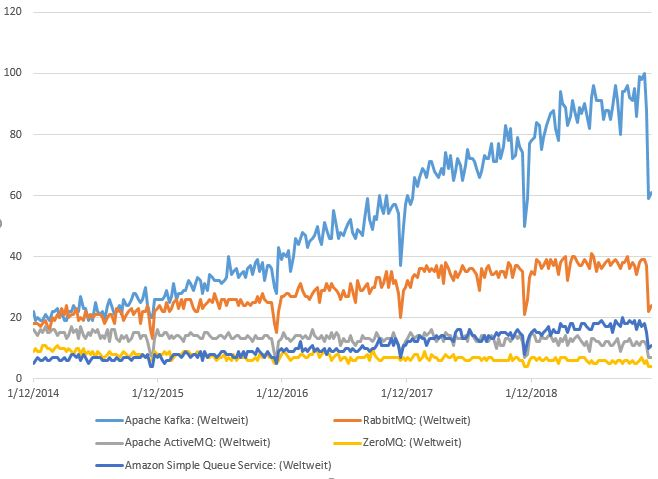
\includegraphics[width=.8\textwidth]{figures/searchinterest.JPG}
	\caption{Relatives Suchinteresse in 5 Jahren; Quelle: Google Trends}
	\label{searchinterest}
\end{figure}
